\subsection{Description and Preparation}

The main difference from the previous dataset is represented by the presence of complex ($\C$) values in certain variables.
In particular the truncation levels and the \texttt{exp} label have all complex values.
Moreover there are additional variables which label the solutions such as the level \texttt{k} and the quantum numbers \texttt{j} and \texttt{m} referring to the \SU{2} representation of the solution.

As in the previous case, the dataset is made of 46 vector-like entries which have to be flattened in the tidy version of the dataset.
The length of the solutions is different in each entry.
The number of solutions for different sizes is summarised in \Cref{fig:wzw:length}.

\begin{figure}[htbp]
  \centering
  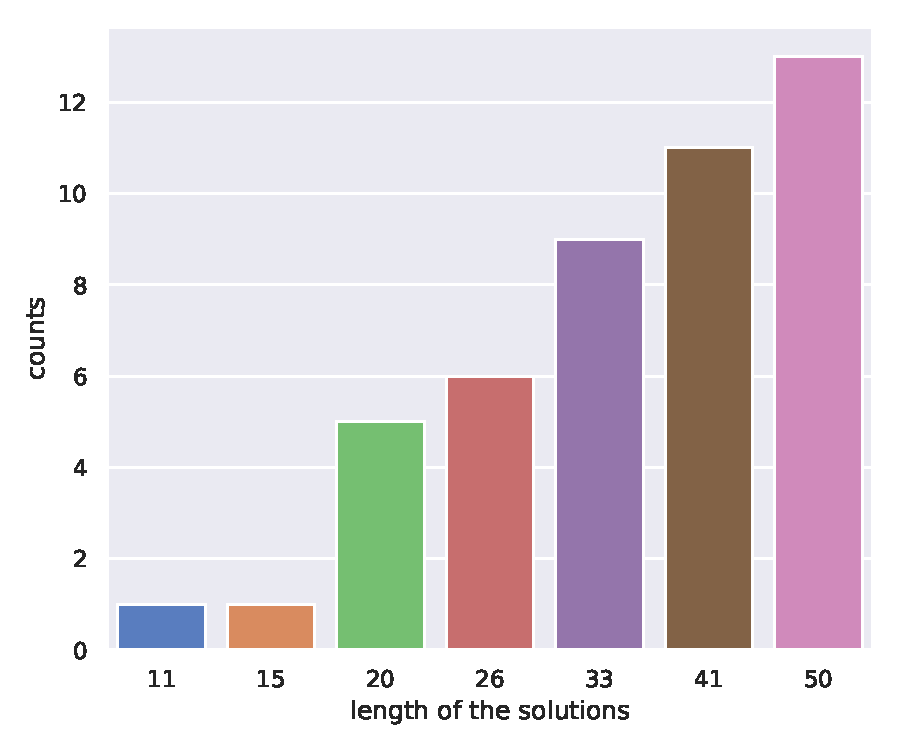
\includegraphics[width=0.6\textwidth]{img/re_sol_length}
  \caption{Length of various solutions.}
  \label{fig:wzw:length}
\end{figure}

In this case the available truncation levels start from the 2nd to the 14th, but since the last 4 levels have mostly empty values (\texttt{level\_11} has only 15 values, while higher levels have only one or two values) we drop them and stop at level 10.
We finally prune the dataset of the duplicates and drop 33 entries (or roughly \SI{2}{\percent} of the total dataset) which are identical over all the variables.

The tidy dataset has therefore 1680 row entries and spans 25 variables including the real and imaginary parts of the label \texttt{exp}, the real and imaginary parts of the truncation levels, \texttt{k}, \texttt{weight}, \texttt{j} and \texttt{m}.


\subsection{Exploratory Data Analysis}

In the exploratory data analysis we mainly focus on the distribution of the values and patterns in the data.
We also look for outliers and relations between the data.


\subsubsection{Distribution of the Data}

Looking at the summary of the data we recognise immediately some properties of the solutions.
In \Cref{fig:wzw:summary} we show a visual summary of the statistics associated with the variables labelling each solutions (without the truncation levels which will be studied later).\footnotemark{}
\footnotetext{%
  In the heatmap values have been normalised by their maximum value in order to be in the range $[-1, 1]$.
}
For instance we immediately recognise that both sum and average of the quantum number \texttt{m} are vanishing, together with possible correlations between \texttt{k}, \texttt{j} and \texttt{weight}.\footnotemark{}
\footnotetext{%
  In fact \texttt{weight} $= \frac{j(j+1)}{k + 2}$.
}

\begin{figure}[htbp]
  \centering
  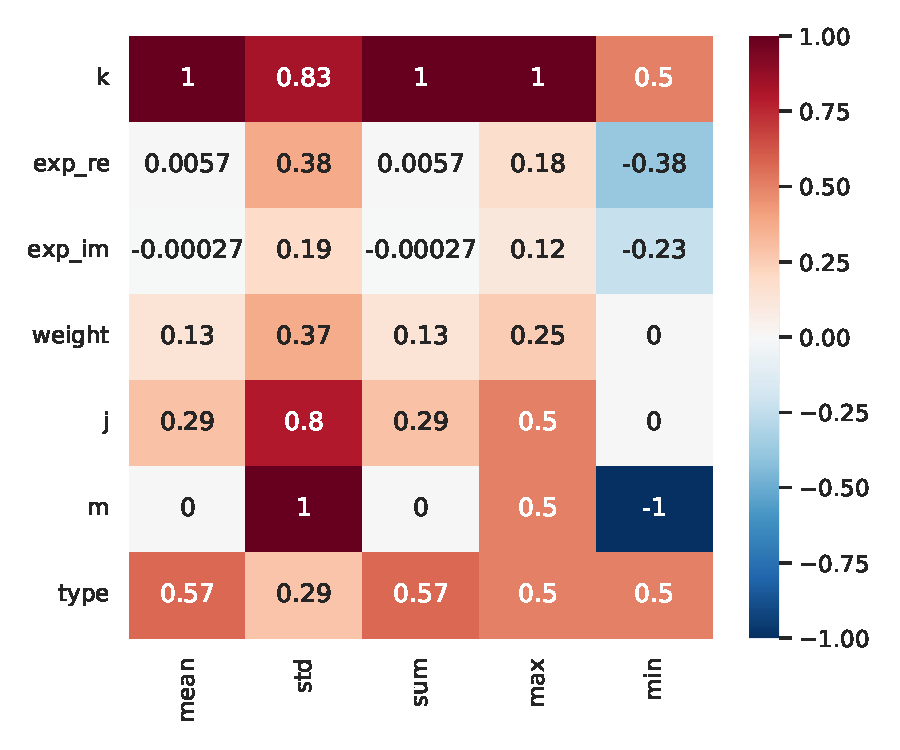
\includegraphics[width=0.6\textwidth]{img/oth_nodup_summary_norm}
  \caption{Visual representation of the summary statistics (normalised by their maximum value).}
  \label{fig:wzw:summary}
\end{figure}

\begin{figure}[htbp]
  \centering
  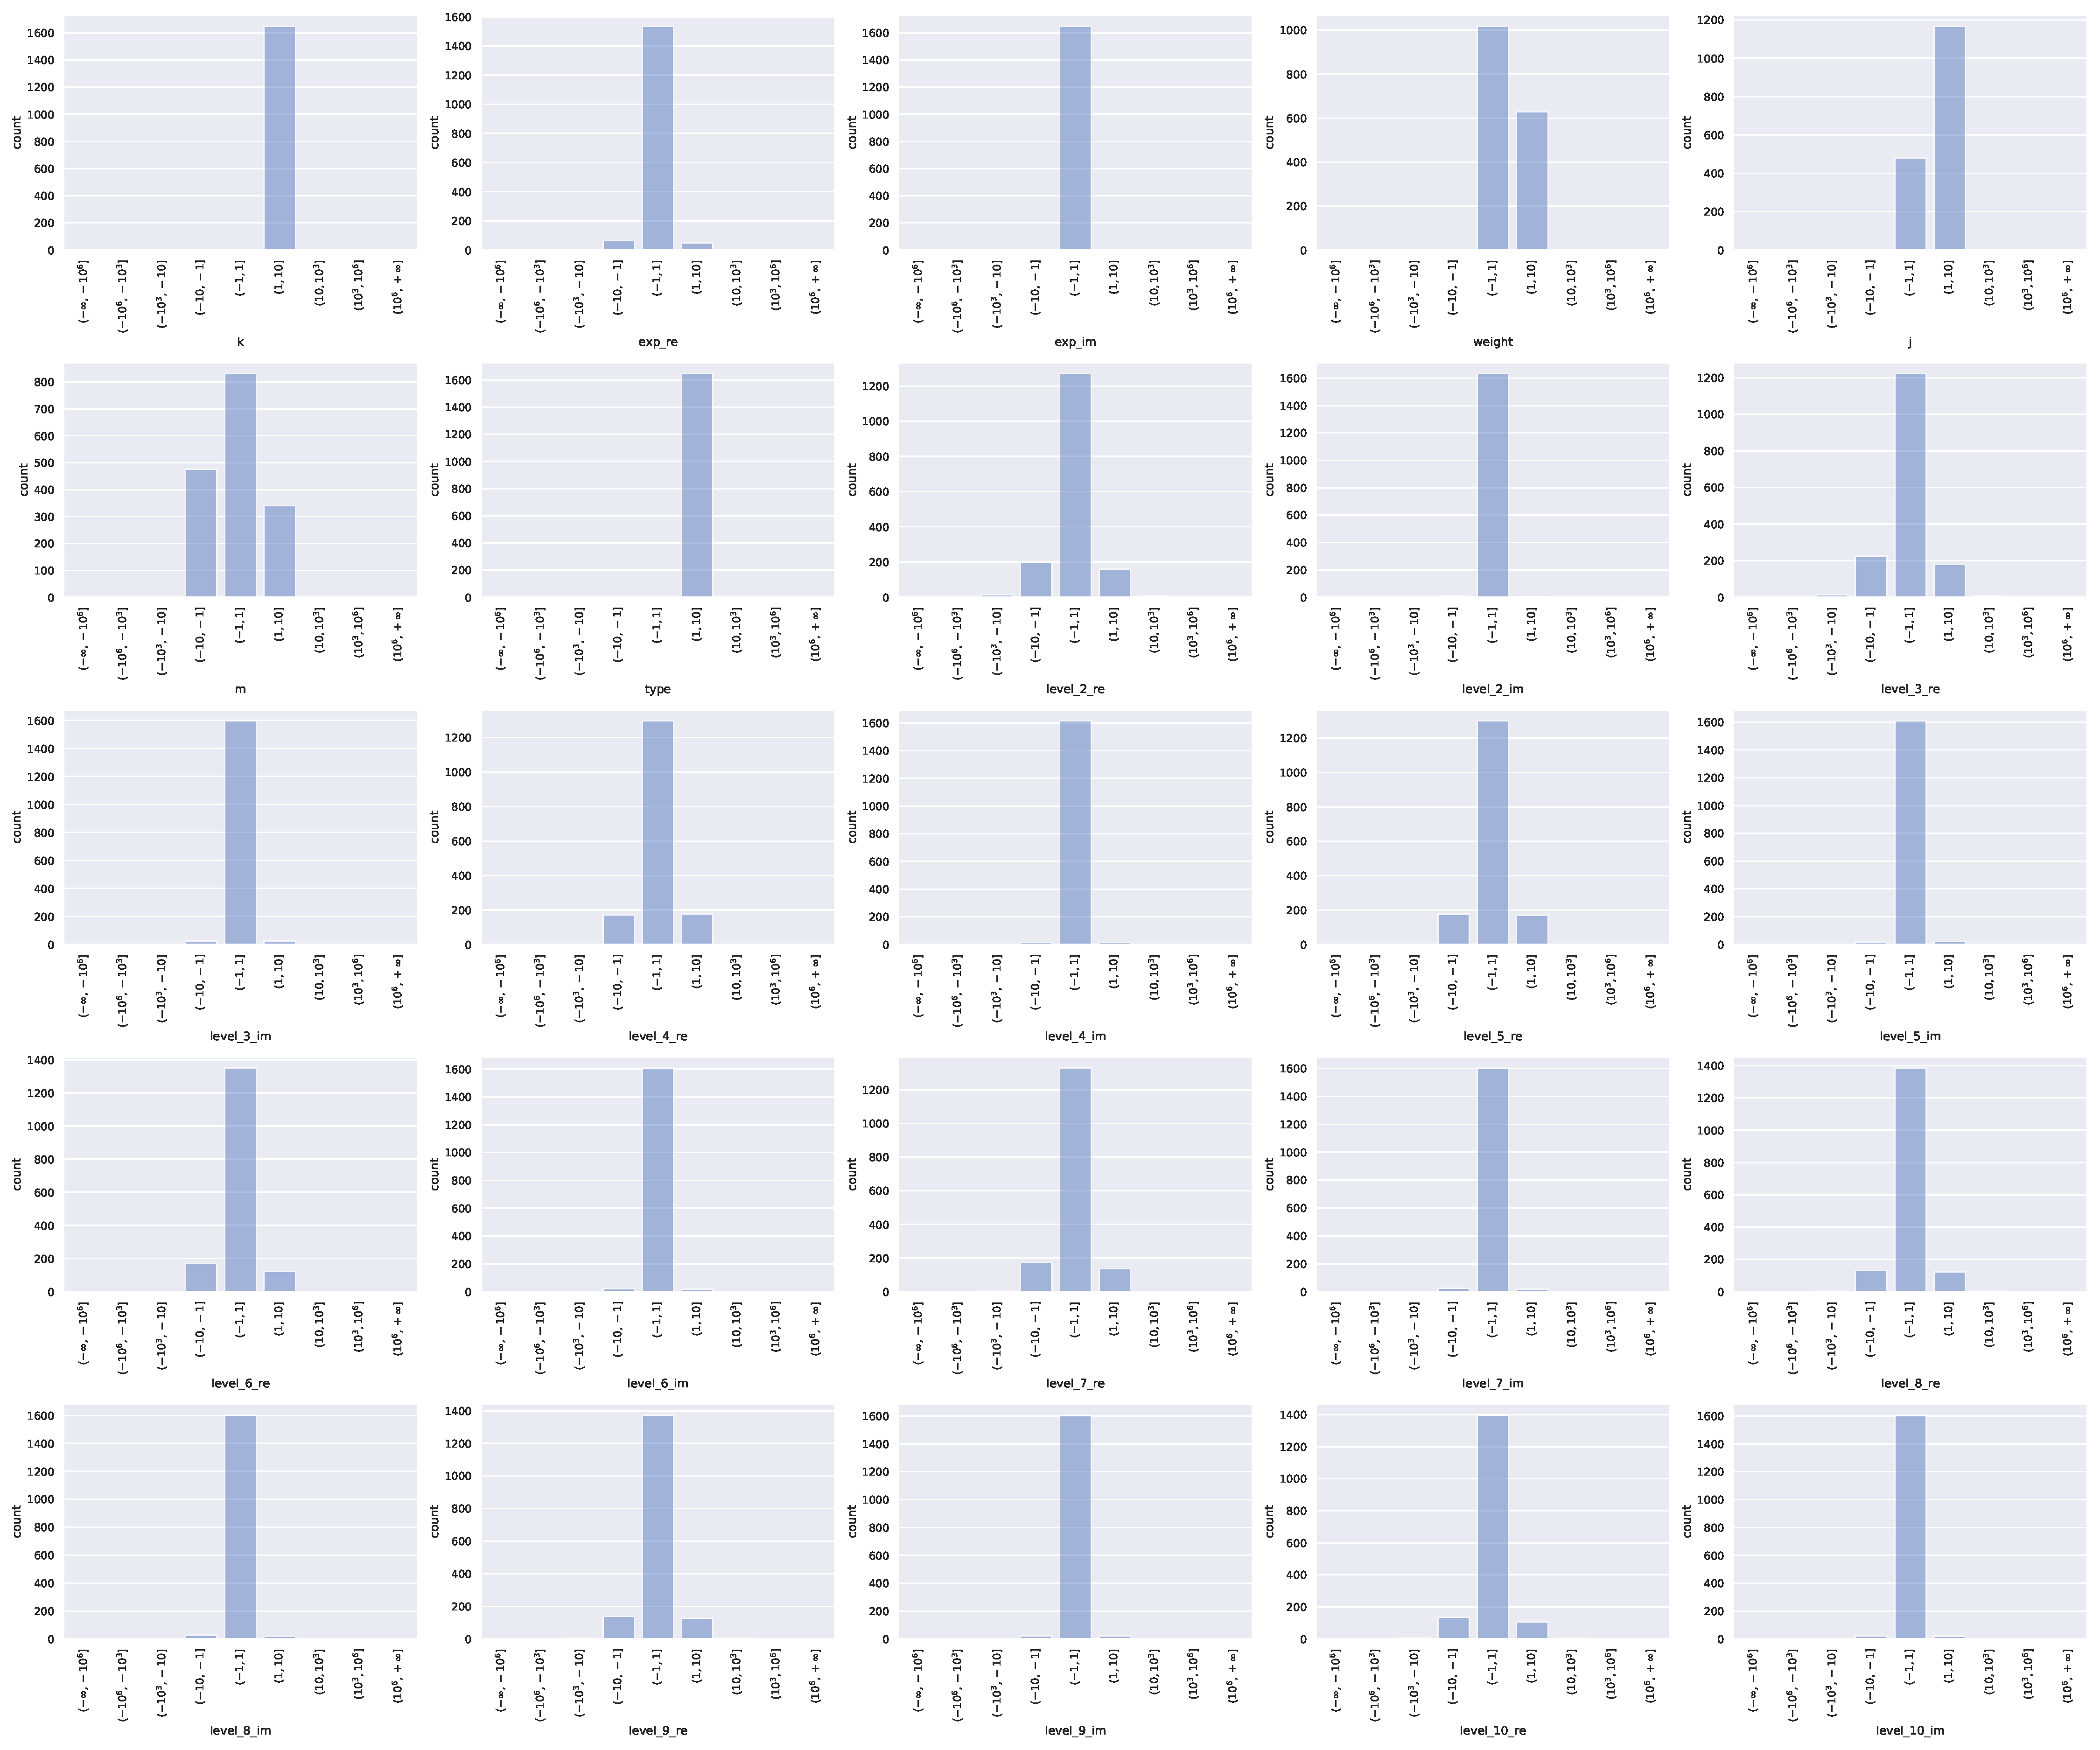
\includegraphics[width=0.6\textwidth]{img/var_counts}
  \caption{Distribution of the variables per order of magnitude.}
  \label{fig:wzw:counts}
\end{figure}


\subsubsection{Outliers Distribution}

Differently from the previous dataset the distribution of the variables is however more balanced (see \Cref{fig:wzw:counts}), even though the fraction of outliers is much larger than before.
However the large number of outliers is mainly due to the presence of non vanishing imaginary part in the truncation levels: only a small number of them is not a real number, thus the average of the imaginary part is narrowly peaked at 0 and any non vanishing contributions is an outlier (see \Cref{fig:wzw:outliers}).

\begin{figure}[htbp]
  \centering
  \begin{subfigure}{0.45\textwidth}
    \centering
    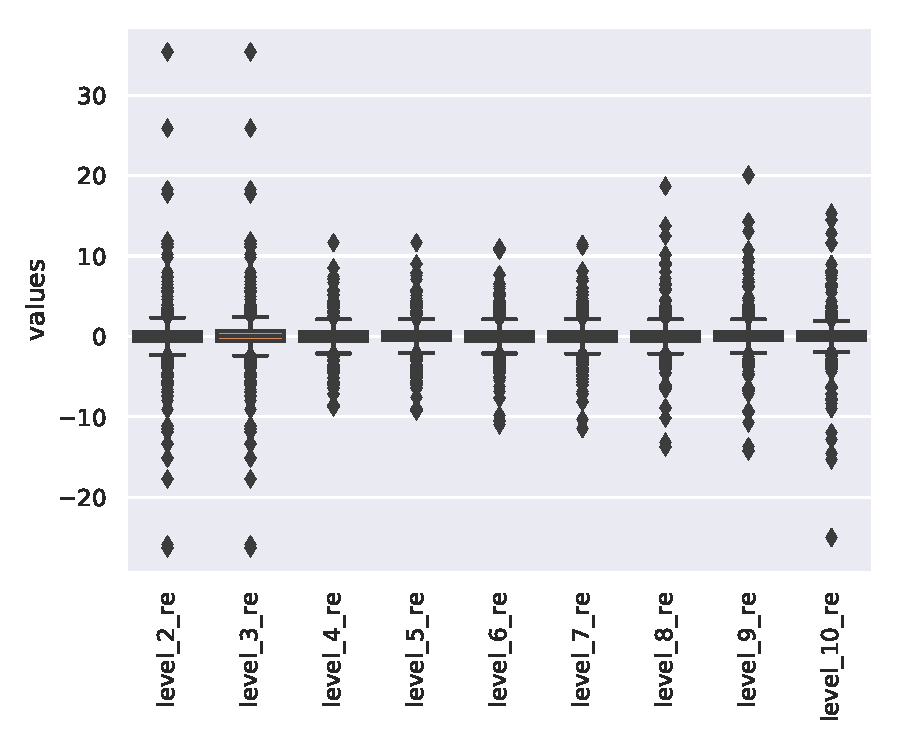
\includegraphics[width=\linewidth]{img/var_box_re}
    \caption{Real part.}
  \end{subfigure}
  \begin{subfigure}{0.45\textwidth}
    \centering
    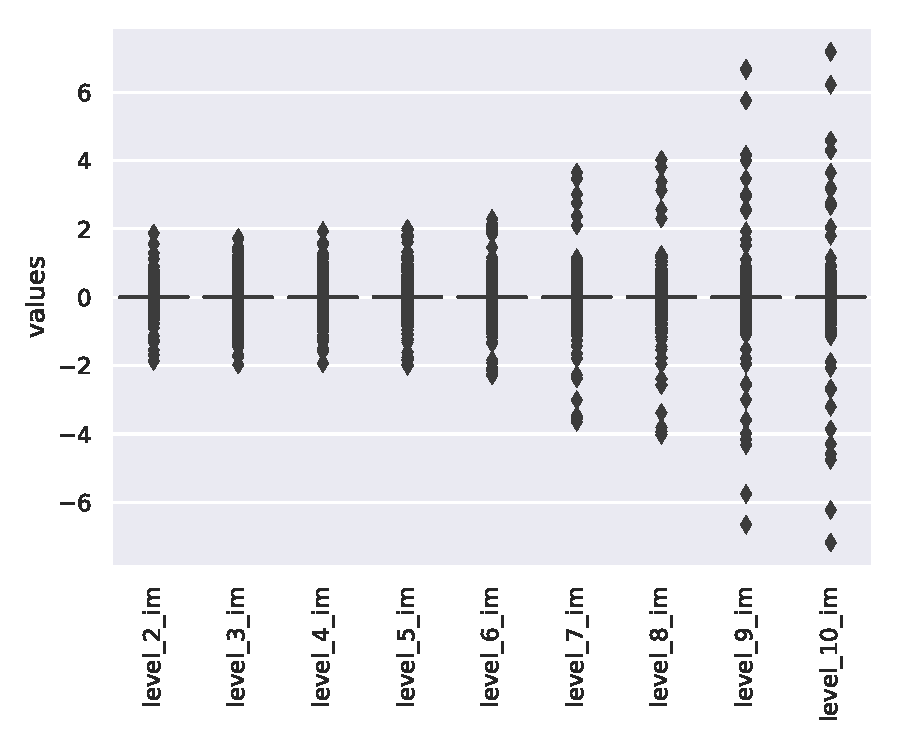
\includegraphics[width=\linewidth]{img/var_box_im}
    \caption{Imaginary part.}
  \end{subfigure}
  \caption{Outlier distribution.}
  \label{fig:wzw:outliers}
\end{figure}

As in the previous dataset there are however strong relations between the data which have been summarised in \Cref{tab:wzw:quantum}.
In particular we have:
\begin{itemize}
  \item \texttt{weight} $\ge 1.0$ and \texttt{type} $= 4$ and \texttt{k} $\in \lbrace 2, 3 \rbrace$ $\Rightarrow$ \texttt{weight} $= 1$ and \texttt{j} $= 0$ and \texttt{m} $= 0$,

  \item \texttt{weight} $\ge 1.0$ and \texttt{type} $= 4$ and \texttt{k} $= 4$ $\Rightarrow$ \texttt{weight} $= 1$,

  \item \texttt{type} $= 2$ $\Rightarrow$ \texttt{weight} $= 0$ and \texttt{j} $= 0$ and \texttt{m} $= 0$.
\end{itemize}

\begin{table}[htbp]
  \centering
  %\resizebox{\textwidth}{!}{%
  \begin{tabular}{@{}ccccccccc@{}}
  \toprule
                             &                    &            & \multicolumn{2}{c}{\textbf{weight}} & \multicolumn{2}{c}{\textbf{j}} & \multicolumn{2}{c}{\textbf{m}} \\
  \textbf{weight}            & \textbf{type}      & \textbf{k} & \textit{mean}     & \textit{var}    & \textit{mean}  & \textit{var}  & \textit{mean}  & \textit{var}  \\ \midrule
  \multirow{7}{*}{$\ge 1.0$} & \multirow{7}{*}{4} & 2          & 1.00              & 0.000           & 0.00           & 0.00          & 0.0            & 0.00          \\
                             &                    & 3          & 1.00              & 0.000           & 0.00           & 0.00          & 0.0            & 0.00          \\
                             &                    & 4          & 1.00              & 0.000           & 1.35           & 0.90          & 0.0            & 1.39          \\
                             &                    & 5          & 1.18              & 0.013           & 1.76           & 1.32          & 0.0            & 2.10          \\
                             &                    & 6          & 1.26              & 0.048           & 2.35           & 1.05          & 0.0            & 3.00          \\
                             &                    & 7          & 1.47              & 0.076           & 2.79           & 1.38          & 0.0            & 4.01          \\
                             &                    & 8          & 1.57              & 0.130           & 3.21           & 1.21          & 0.0            & 4.93          \\
  \midrule
  \multirow{14}{*}{$< 1.0$}  & \multirow{7}{*}{2} & 2          & 0.00              & 0.000           & 0.00           & 0.00          & 0.0            & 0.00          \\
                             &                    & 3          & 0.00              & 0.000           & 0.00           & 0.00          & 0.0            & 0.00          \\
                             &                    & 4          & 0.00              & 0.000           & 0.00           & 0.00          & 0.0            & 0.00          \\
                             &                    & 5          & 0.00              & 0.000           & 0.00           & 0.00          & 0.0            & 0.00          \\
                             &                    & 6          & 0.00              & 0.000           & 0.00           & 0.00          & 0.0            & 0.00          \\
                             &                    & 7          & 0.00              & 0.000           & 0.00           & 0.00          & 0.0            & 0.00          \\
                             &                    & 8          & 0.00              & 0.000           & 0.00           & 0.00          & 0.0            & 0.00          \\
  \cmidrule(l){2-9}
                             & \multirow{7}{*}{4} & 2          & 0.31              & 0.047           & 0.67           & 0.17          & 0.0            & 0.50          \\
                             &                    & 3          & 0.45              & 0.083           & 1.00           & 0.28          & 0.0            & 0.83          \\
                             &                    & 4          & 0.38              & 0.053           & 1.00           & 0.26          & 0.0            & 0.77          \\
                             &                    & 5          & 0.50              & 0.090           & 1.33           & 0.39          & 0.0            & 1.18          \\
                             &                    & 6          & 0.44              & 0.071           & 1.33           & 0.40          & 0.0            & 1.14          \\
                             &                    & 7          & 0.56              & 0.108           & 1.67           & 0.56          & 0.0            & 1.67          \\
                             &                    & 8          & 0.50              & 0.089           & 1.66           & 0.56          & 0.0            & 1.64          \\ \bottomrule
  \end{tabular}%
  %}
  \caption{Relations between the weight and type variables, and other quantum numbers.}
  \label{tab:wzw:quantum}
\end{table}


\subsubsection{Correlation Matrix}

Finally we show the correlation matrix of the features in \Cref{fig:wzw:corr}.
From the correlations we can no longer recognise the oscillating behaviour as in the previous case.
However we notice that real and imaginary parts are separately highly correlated features (though they are completely not correlated between them).
Differently from the previous case the \texttt{weight} variable is poorly correlated with the other features, apart from the previously mentioned relation with \texttt{j}.

\begin{figure}[htbp]
  \centering
  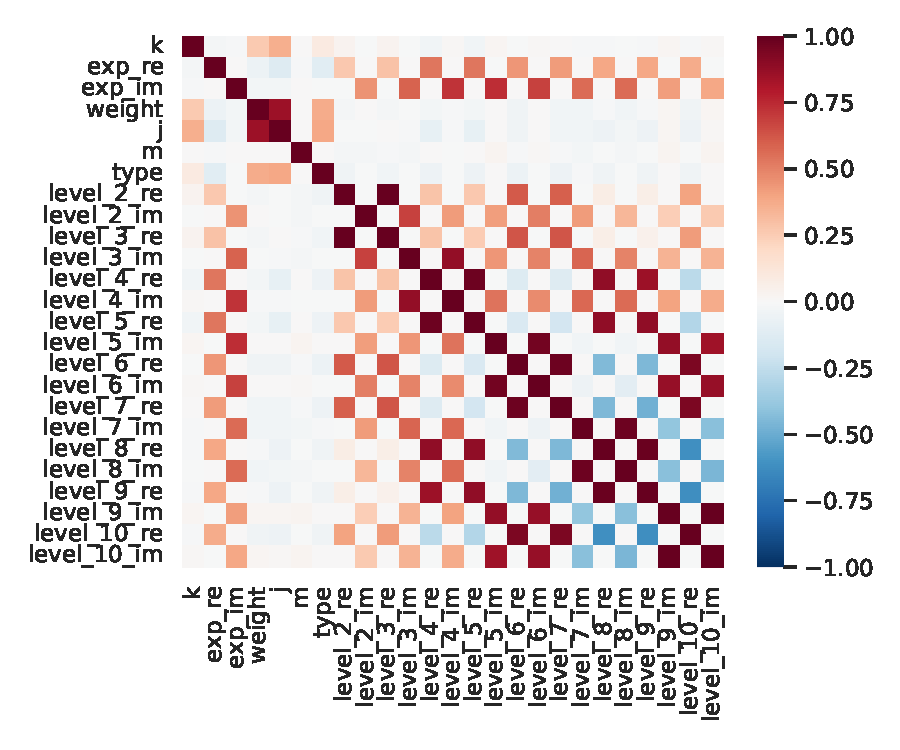
\includegraphics[width=0.6\textwidth]{img/wzw_corr_mat}
  \caption{Correlation matrix of the \wzw model.}
  \label{fig:wzw:corr}
\end{figure}


\subsubsection{Principal Components Analysis}

As in the previous case, we also analyse the principal components of the truncation levels.
We perform the analysis in two separate ways: in the first we consider the whole group of truncation levels and robustly scale them against outliers (using the \texttt{RobustScaler} class in \texttt{Scikit-learn}), in the second we separate real and imaginary parts, standardise the first (using the \texttt{StandardScaler} in \texttt{Scikit-learn}) and robustly scale the latter.
We then perform the same analysis as before.

As we see in \Cref{fig:wzw:svd} after performing the \svd, in both cases a large part of the variance is already captured by one of the principal components (both the whole and separate datasets retain more than \SI{99}{\percent} of the variance with just one component).
It may therefore be possible to use the principal components to have a fixed input size for the algorithms and be compatible with other datasets.

\begin{figure}[htbp]
  \centering
  \begin{subfigure}{0.45\textwidth}
    \centering
    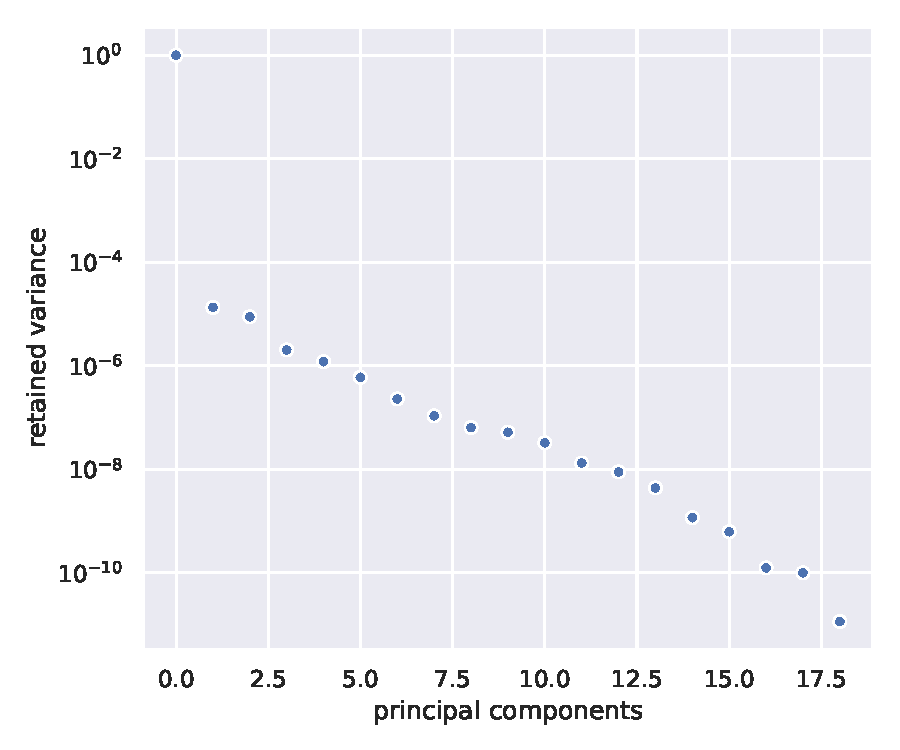
\includegraphics[width=\linewidth]{img/wzw_svd_tot}
    \caption{Whole dataset.}
  \end{subfigure}
  \begin{subfigure}{0.45\textwidth}
    \centering
    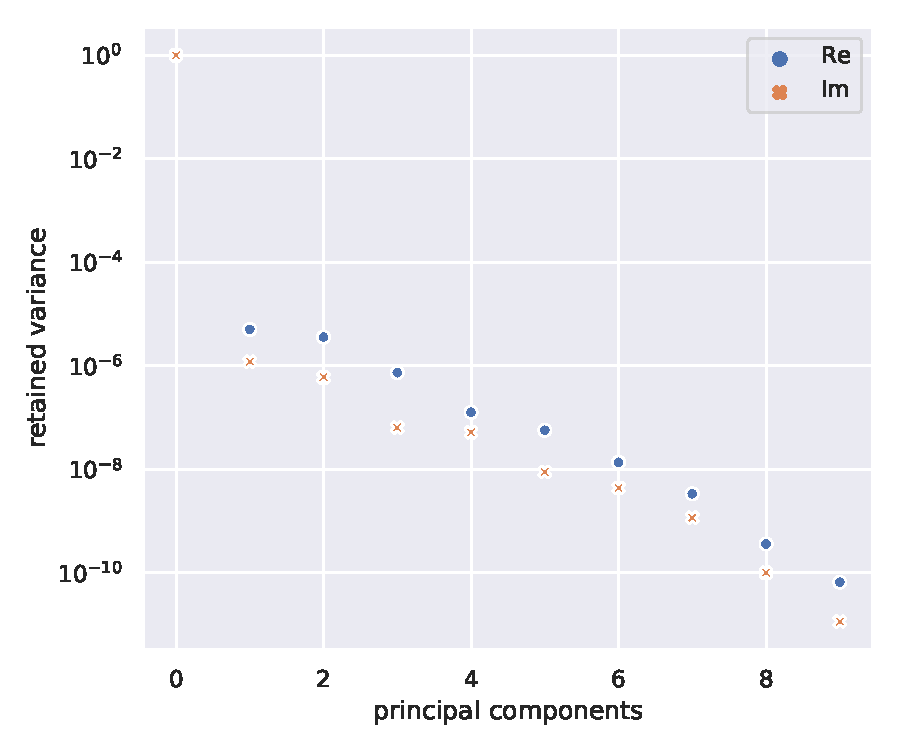
\includegraphics[width=\linewidth]{img/wzw_svd_sep}
    \caption{Separate dataset.}
  \end{subfigure}
  \caption{Principal components of the truncation levels.}
  \label{fig:wzw:svd}
\end{figure}


\subsection{Statistical Inference}

As for the previous case, using the \eda data we performed the \anova on the \wzw model using a simple linear regressor.
For this we used \SI{80}{\percent} of the dataset for training and the rest as development set: since the data is already labelled, we do not need to separate the samples according to the \texttt{solutions} variable.
However in this case we will keep all the variables present in the dataset and perform the regression predicting both the real and imaginary parts of \texttt{exp} simultaneously.
With 313 \dof\ we reached a \mse of 0.06 with a \ci $\left[0.0, 0.07\right]$ and $\rr = 0.83$ (both are better than the previous dataset signalling that features and labels may be more correlated in this case).

\begin{table}[htbp]
  \centering
  \resizebox{\textwidth}{!}{%
  \begin{tabular}{@{}ccccccccc@{}}
  \toprule
                         & \textbf{coeff.\ -- Re}
                         & \textbf{coeff.\ -- Im}
                         & \textbf{std.\ err.\ -- Re}
                         & \textbf{std.\ err.\ -- Im}
                         & \textbf{t -- Re}
                         & \textbf{t -- Im}
                         & \textbf{p-value -- Re}
                         & \textbf{p-value -- Im} \\
  \midrule
  \texttt{k}             & 0.003  & -0.005  & 0.015 & 0.002   & 0.176    & -2.977   & 0.861  & 0.003  \\
  \texttt{weight}        & 0.05   & -0.005  & 0.03  & 0.004   & 1.520    & -1.361   & 0.130  & 0.175  \\
  \texttt{j}             & -0.033 & 0.00035 & 0.015 & 0.0017  & -2.263   & 0.211    & 0.024  & 0.833  \\
  \texttt{m}             & 0.000  & 0.0003  & 0.013 & 0.0014  & 0.075    & 0.230    & 0.940  & 0.818  \\
  \texttt{type}          & 0.00   & 0.010   & 0.04  & 0.0047  & 0.058    & 2.234    & 0.954  & 0.026  \\
  \texttt{Re(level 2)}   & 0.329  & 0.0088  & 0.006 & 0.0007  & 51.791   & 12.163   & 0.000  & 0.000  \\
  \texttt{Im(level 2)}   & 0.02   & -0.034  & 0.09  & 0.011   & 0.265    & -3.271   & 0.791  & 0.001  \\
  \texttt{Re(level 3)}   & -0.349 & -0.0086 & 0.006 & 0.0007  & -55.653  & -12.120  & 0.000  & 0.000  \\
  \texttt{Im(level 3)}   & -0.07  & -0.064  & 0.05  & 0.006   & -1.242   & -10.764  & 0.215  & 0.000  \\
  \texttt{Re(level 4)}   & -0.516 & 0.0145  & 0.015 & 0.0017  & -35.415  & 8.785    & 0.000  & 0.000  \\
  \texttt{Im(level 4)}   & 0.11   & 0.062   & 0.06  & 0.006   & 1.890    & 9.801    & 0.060  & 0.000  \\
  \texttt{Re(level 5)}   & -0.036 & -0.0175 & 0.014 & 0.0016  & -2.519   & -10.871  & 0.012  & 0.000  \\
  \texttt{Im(level 5)}   & -0.10  & -1.507  & 0.05  & 0.006   & -2.019   & -267.397 & 0.044  & 0.000  \\
  \texttt{Re(level 6)}   & -4.931 & -0.0256 & 0.014 & 0.0016  & -340.537 & -15.605  & 0.000  & 0.000  \\
  \texttt{Im(level 6)}   & 0.15   & 1.939   & 0.05  & 0.006   & 2.960    & 346.379  & 0.003  & 0.000  \\
  \texttt{Re(level 7)}   & 4.539  & 0.0262  & 0.014 & 0.0016  & 328.362  & 16.776   & 0.000  & 0.000  \\
  \texttt{Im(level 7)}   & -0.00  & -3.980  & 0.04  & 0.005   & -0.132   & -807.934 & 0.895  & 0.000  \\
  \texttt{Re(level 8)}   & -3.71  & -0.0383 & 0.013 & 0.0015  & -279.284 & -25.439  & 0.000  & 0.000  \\
  \texttt{Im(level 8)}   & -0.04  & 4.444   & 0.04  & 0.005   & -0.991   & 960.701  & 0.322  & 0.000  \\
  \texttt{Re(level 9)}   & 4.684  & 0.0406  & 0.013 & 0.0014  & 367.810  & 28.150   & 0.000  & 0.000  \\
  \texttt{Im(level 9)}   & 0.08   & -2.587  & 0.03  & 0.003   & 2.756    & -775.714 & 0.006  & 0.000  \\
  \texttt{Re(level 10)}  & 0.874  & 0.0009  & 0.012 & 0.0013  & 75.406   & 0.693    & 0.000  & 0.489  \\
  \texttt{Im(level 10)}  & -0.14  & 2.687   & 0.03  & 0.003   & -4.800   & 840.827  & 0.000  & 0.000  \\                                                  
  \bottomrule
  \end{tabular}%
  }
  \caption{Results of the \anova on the linear model.}
  \label{tab:wzw:anova}
\end{table}

In \Cref{tab:wzw:anova} we show the results of the analysis: we show the choice of the coefficients and their statistics in separate columns for the real and imaginary parts of \texttt{exp}).
Differently from the previous case the data is a bit more complex and in some cases it shows that we could actually drop some of the variables.
For instance we will certainly drop \texttt{k} which does not seem to influence the final result (its p-value is very high).
Curiously enough, it seems that in order to predict $\Re(exp)$ we could just use the real parts of the variables in the dataset, while the situation for $\Im(exp)$ requires the contributions of both real and imaginary parts of the input features.


\subsection{Model Dependent Deep Learning Analysis}


As a prosecution of the exploratory analysis we also performed a prediction analysis using the same ANN model used for the previous dataset.
The necessary modifications however concern the input shape of the architecture (here we have more input variables) and the output layer: we are interested in predicting both real and imaginary parts of the output at the same time.
This in turn will not be necessary for the aggregate analysis but it might be worth noting the results.

For the learning model we split the dataset into \SI{80}{\percent} for training, \SI{10}{\percent} for validation and the remaining \SI{10}{\percent} as a test set.
In general the ANN model behaved extremely well in the training and validation folds, while it performed poorly in the test set: the \rr score for both $\Re(exp)$ and $\Im(exp)$ dropped respectively to \num{0.66} and \num{0.30} in the test set while it was above \num{0.94} in both training and validation folds.\footnotemark{}
\footnotetext{%
  As a consequence also the \mse plummeted in the test set.
}
This however seems to be entirely due to a small number of samples in the test set which drove away the \mse and the \rr score with respect to the validation and training sets.
In \Cref{fig:wzw:preds} we can clearly see the sample (the same between real and imaginary parts) spoiling the result.

\begin{figure}[htbp]
  \centering
  \begin{subfigure}{0.45\textwidth}
    \centering
    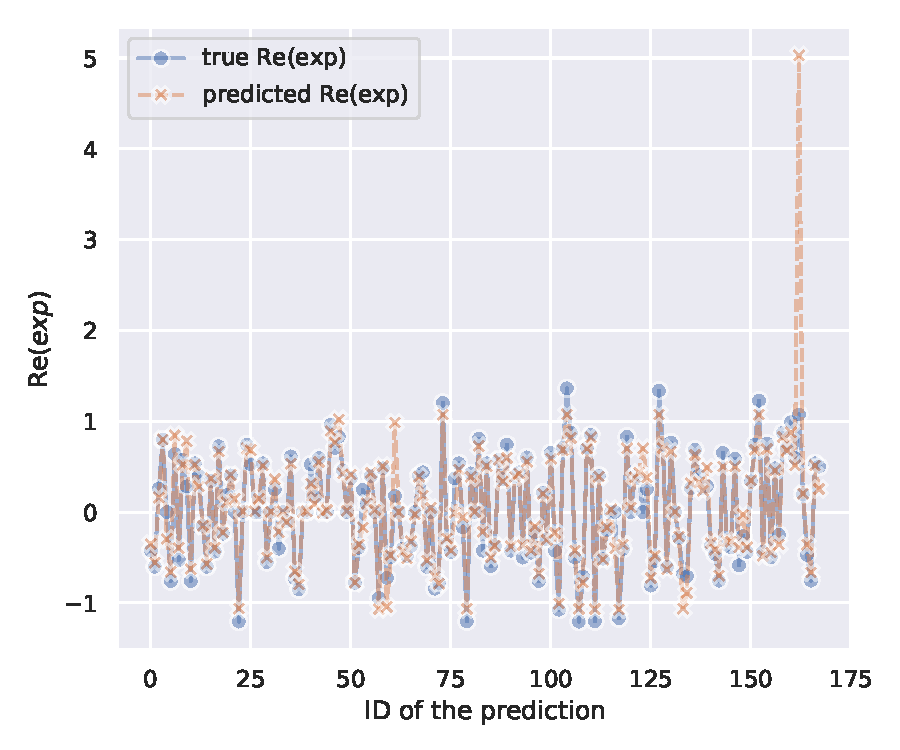
\includegraphics[width=\linewidth]{img/ann_model_test_re_lineplot}
    \caption{Real part.}
  \end{subfigure}
  \begin{subfigure}{0.45\textwidth}
    \centering
    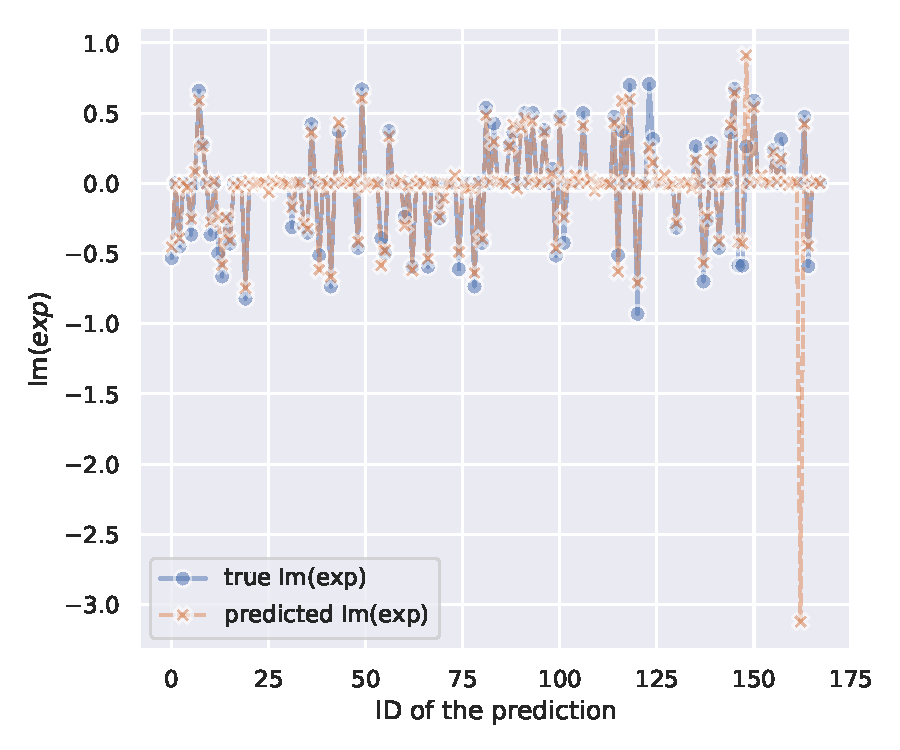
\includegraphics[width=\linewidth]{img/ann_model_test_im_lineplot}
    \caption{Imaginary part.}
  \end{subfigure}
  \caption{Predictions and true values of the \texttt{exp} label.}
  \label{fig:wzw:preds}
\end{figure}


\subsection{Fourier Analysis and Signal Processing}

As in the case of the lumps dataset we proceed to the analysis of the WZW dataset using Fourier analysis.
In general we use the same prescriptions as in the lumps dataset as far as validation techniques and metrics used in the analysis.
The main difference between the datasets is the fact that the WZW truncation levels are in general complex numbers: when computing the Fourier Transform we use the \texttt{np.fft.fft} method in \texttt{numpy}.
We also consider the complex modulus and the argument angle of the \texttt{exp} label as totally independent, since it should be possible to compute combinations of the observables such that they are purely real numbers.


\subsubsection{Tidying the Dataset}

Differently from the analysis of this section, for the Fourier analysis we need to be more careful when tidying the dataset.
As a matter of fact we cannot include complex conjugate observables which would duplicate the entries in Fourier space.
In fact we consider as duplicates all samples having the same label \texttt{k}, same \texttt{weight}, same \SU{2} quantum numbers \texttt{j} and \texttt{m}, same complex modulus of the \texttt{exp} label, and the same absolute value of its argument angle (since its value is in the interval $[-1, 1]$ after dividing it by a factor $\pi$).
The fraction of duplicates with this separation is \SI{45.7}{\percent}.
The final dataset is made of \num{912} entries.


\subsubsection{Training and Results}

As in the lumps dataset we first compute the Fourier Transform of the truncation levels and then apply the standard scaler.
The input features of the \ml models will therefore be the scaled complex modulus and the scaled angles of the truncation levels, the \texttt{weight} of the observables and their \texttt{type}.

We train a linear model with $\ell_2$ regularisation, a SVM with Gaussian kernel, a GBDT model and an ANN.
For the first three models we use the Bayes optimisation of the hyperparameters using the \mse as scoring function.
In the case of the ANN the optimisation is done by hand.

The ANN model used in this first analysis is a fully connected architecture.
For both the complex modulus and the angle of \texttt{exp} the ANN is made of \num{6} hidden layer with \numlist{50;30;20;20;10;10} units each.
We used a \texttt{LeakyReLU} activation function after each of them (\num{0.05} as slope factor).
We also included a \num{0.03} dropout rate after the first layer and \num{0.05} for the subsequent three layers.
In the case of the complex modulus of \texttt{exp} we also implemented a factor $10^{-5}$ as $\ell_2$ regularisation of the kernel matrix in each hidden layer.
For both architectures we use the \texttt{Adam} optimizer with an initial learning rate $lr_0 = 10^{-3}$.
We then use a learning rate scheduler to reduce the learning rate as in~\eqref{eq:lumps:lrschedule}.
We also use an early stopping callback after \num{2500} epochs without improvement on the validation loss function (\mse).

\begin{table}[htbp]
  \centering
  %\resizebox{\textwidth}{!}{%
  \begin{tabular}{@{}ccccc@{}}
       \toprule
       & \mse & \mae & \rr & R \\
       \midrule
    LR   & 0.08 & 0.23 & 0.07 & 0.50 \\
    SVR  & 0.04 & 0.15 & 0.54 & 0.32 \\
    GBDT & 0.03 & 0.13 & 0.70 & 0.29 \\
    ANN  & 0.05 & 0.15 & 0.48 & 0.22 \\
       \bottomrule
  \end{tabular}%
  %}
  \caption{%
    Predictions of the \ml analysis trained the entire WZW dataset.
    Results refer to the complex modulus of the test fold.
  }
  \label{tab:wzw:fftres_mod}
\end{table}

\begin{table}[htbp]
  \centering
  %\resizebox{\textwidth}{!}{%
  \begin{tabular}{@{}ccccc@{}}
       \toprule
       & \mse & \mae & \rr & R \\
       \midrule
    LR   & 0.24 & 0.42 & 0.16 & 2.96 \\
    SVR  & 0.20 & 0.33 & 0.30 & 2.75 \\
    GBDT & 0.08 & 0.18 & 0.72 & 2.35 \\
    ANN  & 0.14 & 0.19 & 0.53 & 2.67 \\
       \bottomrule
  \end{tabular}%
  %}
  \caption{%
    Predictions of the \ml analysis trained the entire WZW dataset.
    Results refer to the argument angle of the test fold.
  }
  \label{tab:wzw:fftres_ang}
\end{table}

In~\Cref{tab:wzw:fftres_mod} and \Cref{tab:wzw:fftres_ang} we show the metrics computed on the test fold for the complex modulus and the argument angle of \texttt{exp} respectively.
In general it seems that the Fourier analysis does not help the predictions in the WZW model when using the traditional approach.
In~\Cref{fig:wzw:reshist_mod} we show the univariate distributions of the residuals and the logarithm of the ratio between the predicted residual $y_{\text{true}} - y_{\text{pred}}$ and the finite residual $y_{\text{true}} - y_{\text{finite}}$ where $y_{\text{finite}}$ are the values of the complex modulus of the variable \texttt{level\_10} in this case.
In~\Cref{fig:wzw:reshist_ang} we show the same distributions for the angle of the label.

\begin{figure}[htbp]
  \centering
  \begin{subfigure}[b]{0.45\linewidth}
    \centering
    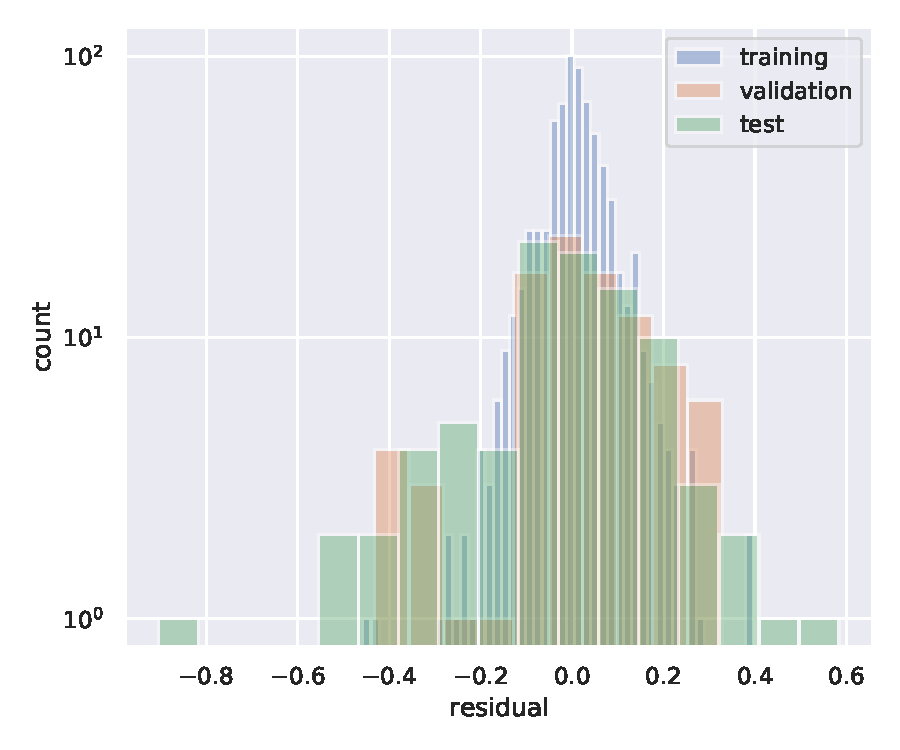
\includegraphics[width=\linewidth]{img/wzw_ann_residual_histogram_compare_mod}
    \caption{Residuals.}
  \end{subfigure}
  \begin{subfigure}[b]{0.45\linewidth}
    \centering
    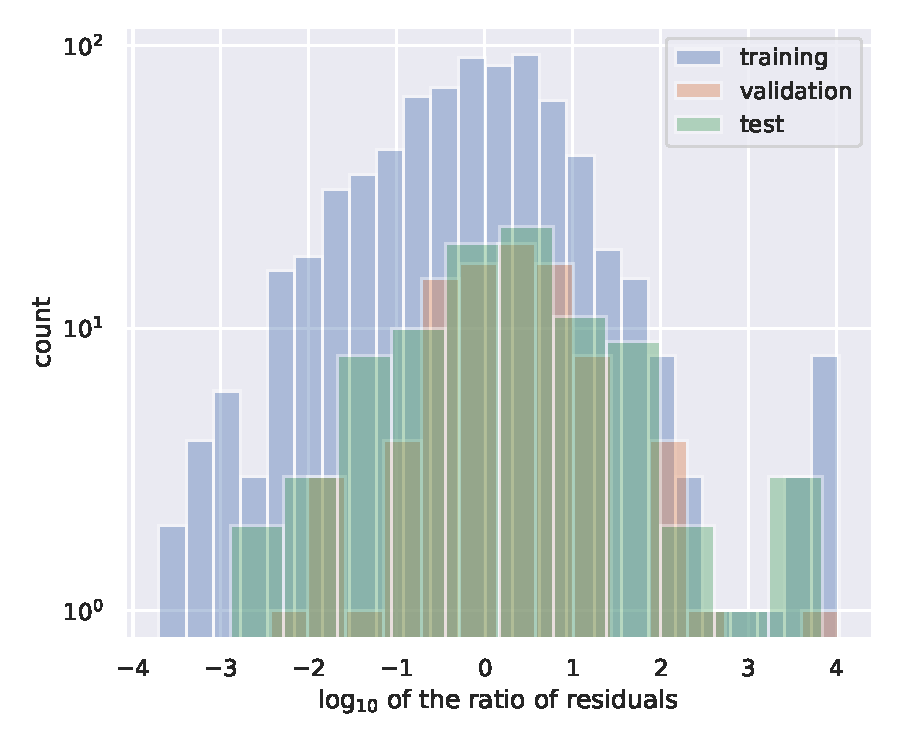
\includegraphics[width=\linewidth]{img/wzw_ann_ratio_histogram_compare_mod}
    \caption{Logarithm of the ratio of the residuals.}
  \end{subfigure}
  \caption{Residual errors and ratio of the residuals of the complex modulus of \texttt{exp}.}
  \label{fig:wzw:reshist_mod}
\end{figure}

\begin{figure}[htbp]
  \centering
  \begin{subfigure}[b]{0.45\linewidth}
    \centering
    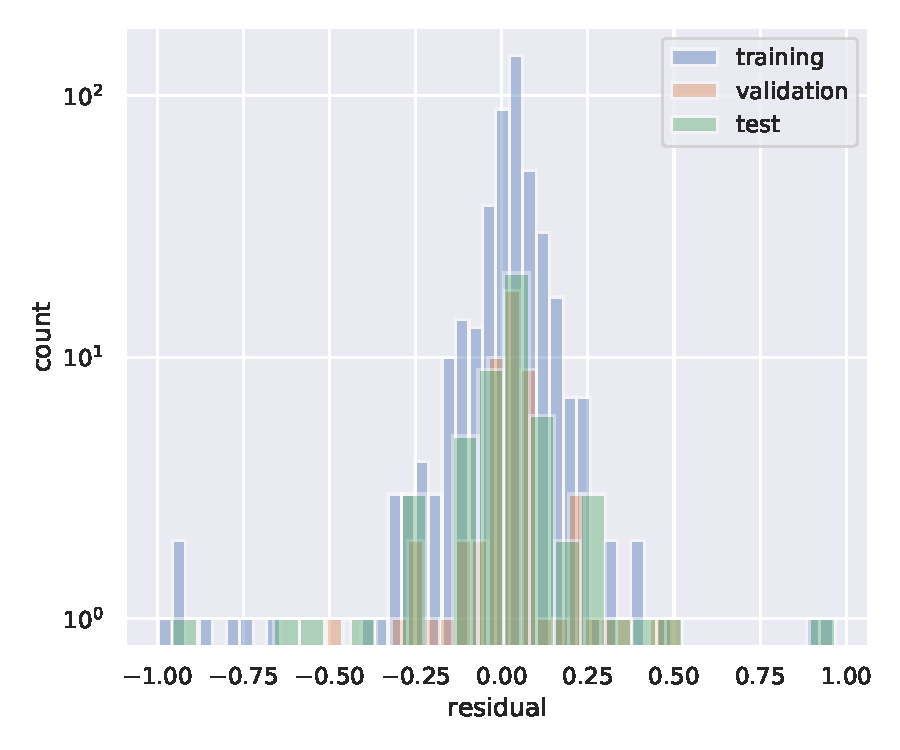
\includegraphics[width=\linewidth]{img/wzw_ann_residual_histogram_compare_angle}
    \caption{Residuals.}
  \end{subfigure}
  \begin{subfigure}[b]{0.45\linewidth}
    \centering
    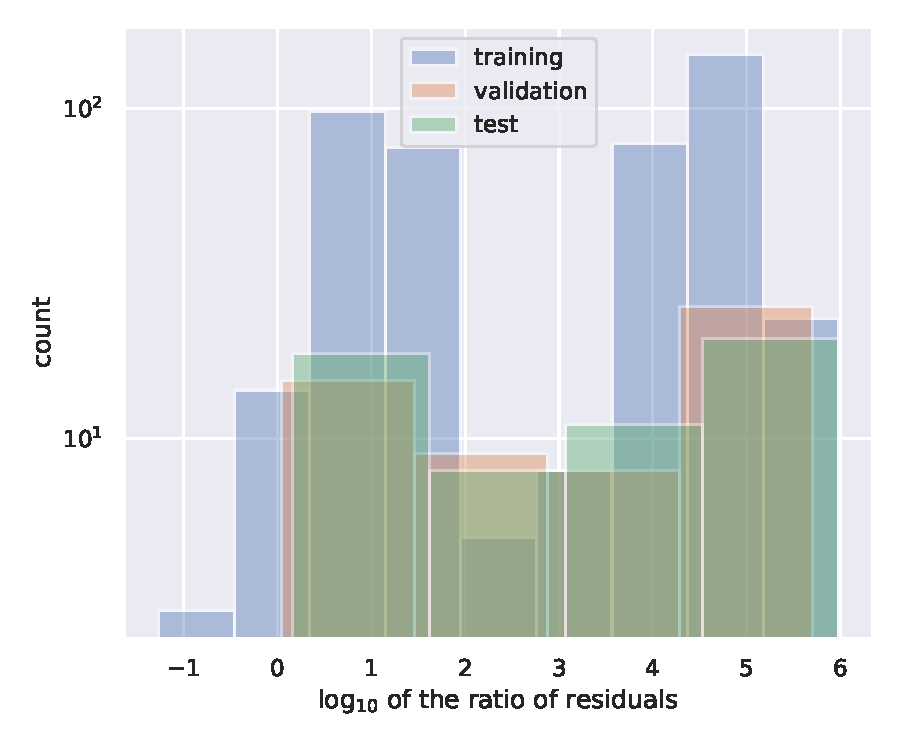
\includegraphics[width=\linewidth]{img/wzw_ann_ratio_histogram_compare_angle}
    \caption{Logarithm of the ratio of the residuals.}
  \end{subfigure}
  \caption{Residual errors and ratio of the residuals of the angle of \texttt{exp}.}
  \label{fig:wzw:reshist_ang}
\end{figure}


\subsubsection{Signal Processing and LSTM Network}

Following the analysis of the lumps dataset, we consider just the truncation levels and process them as a signal to make predictions of the label \texttt{exp}.

\begin{figure}[htbp]
  \centering
  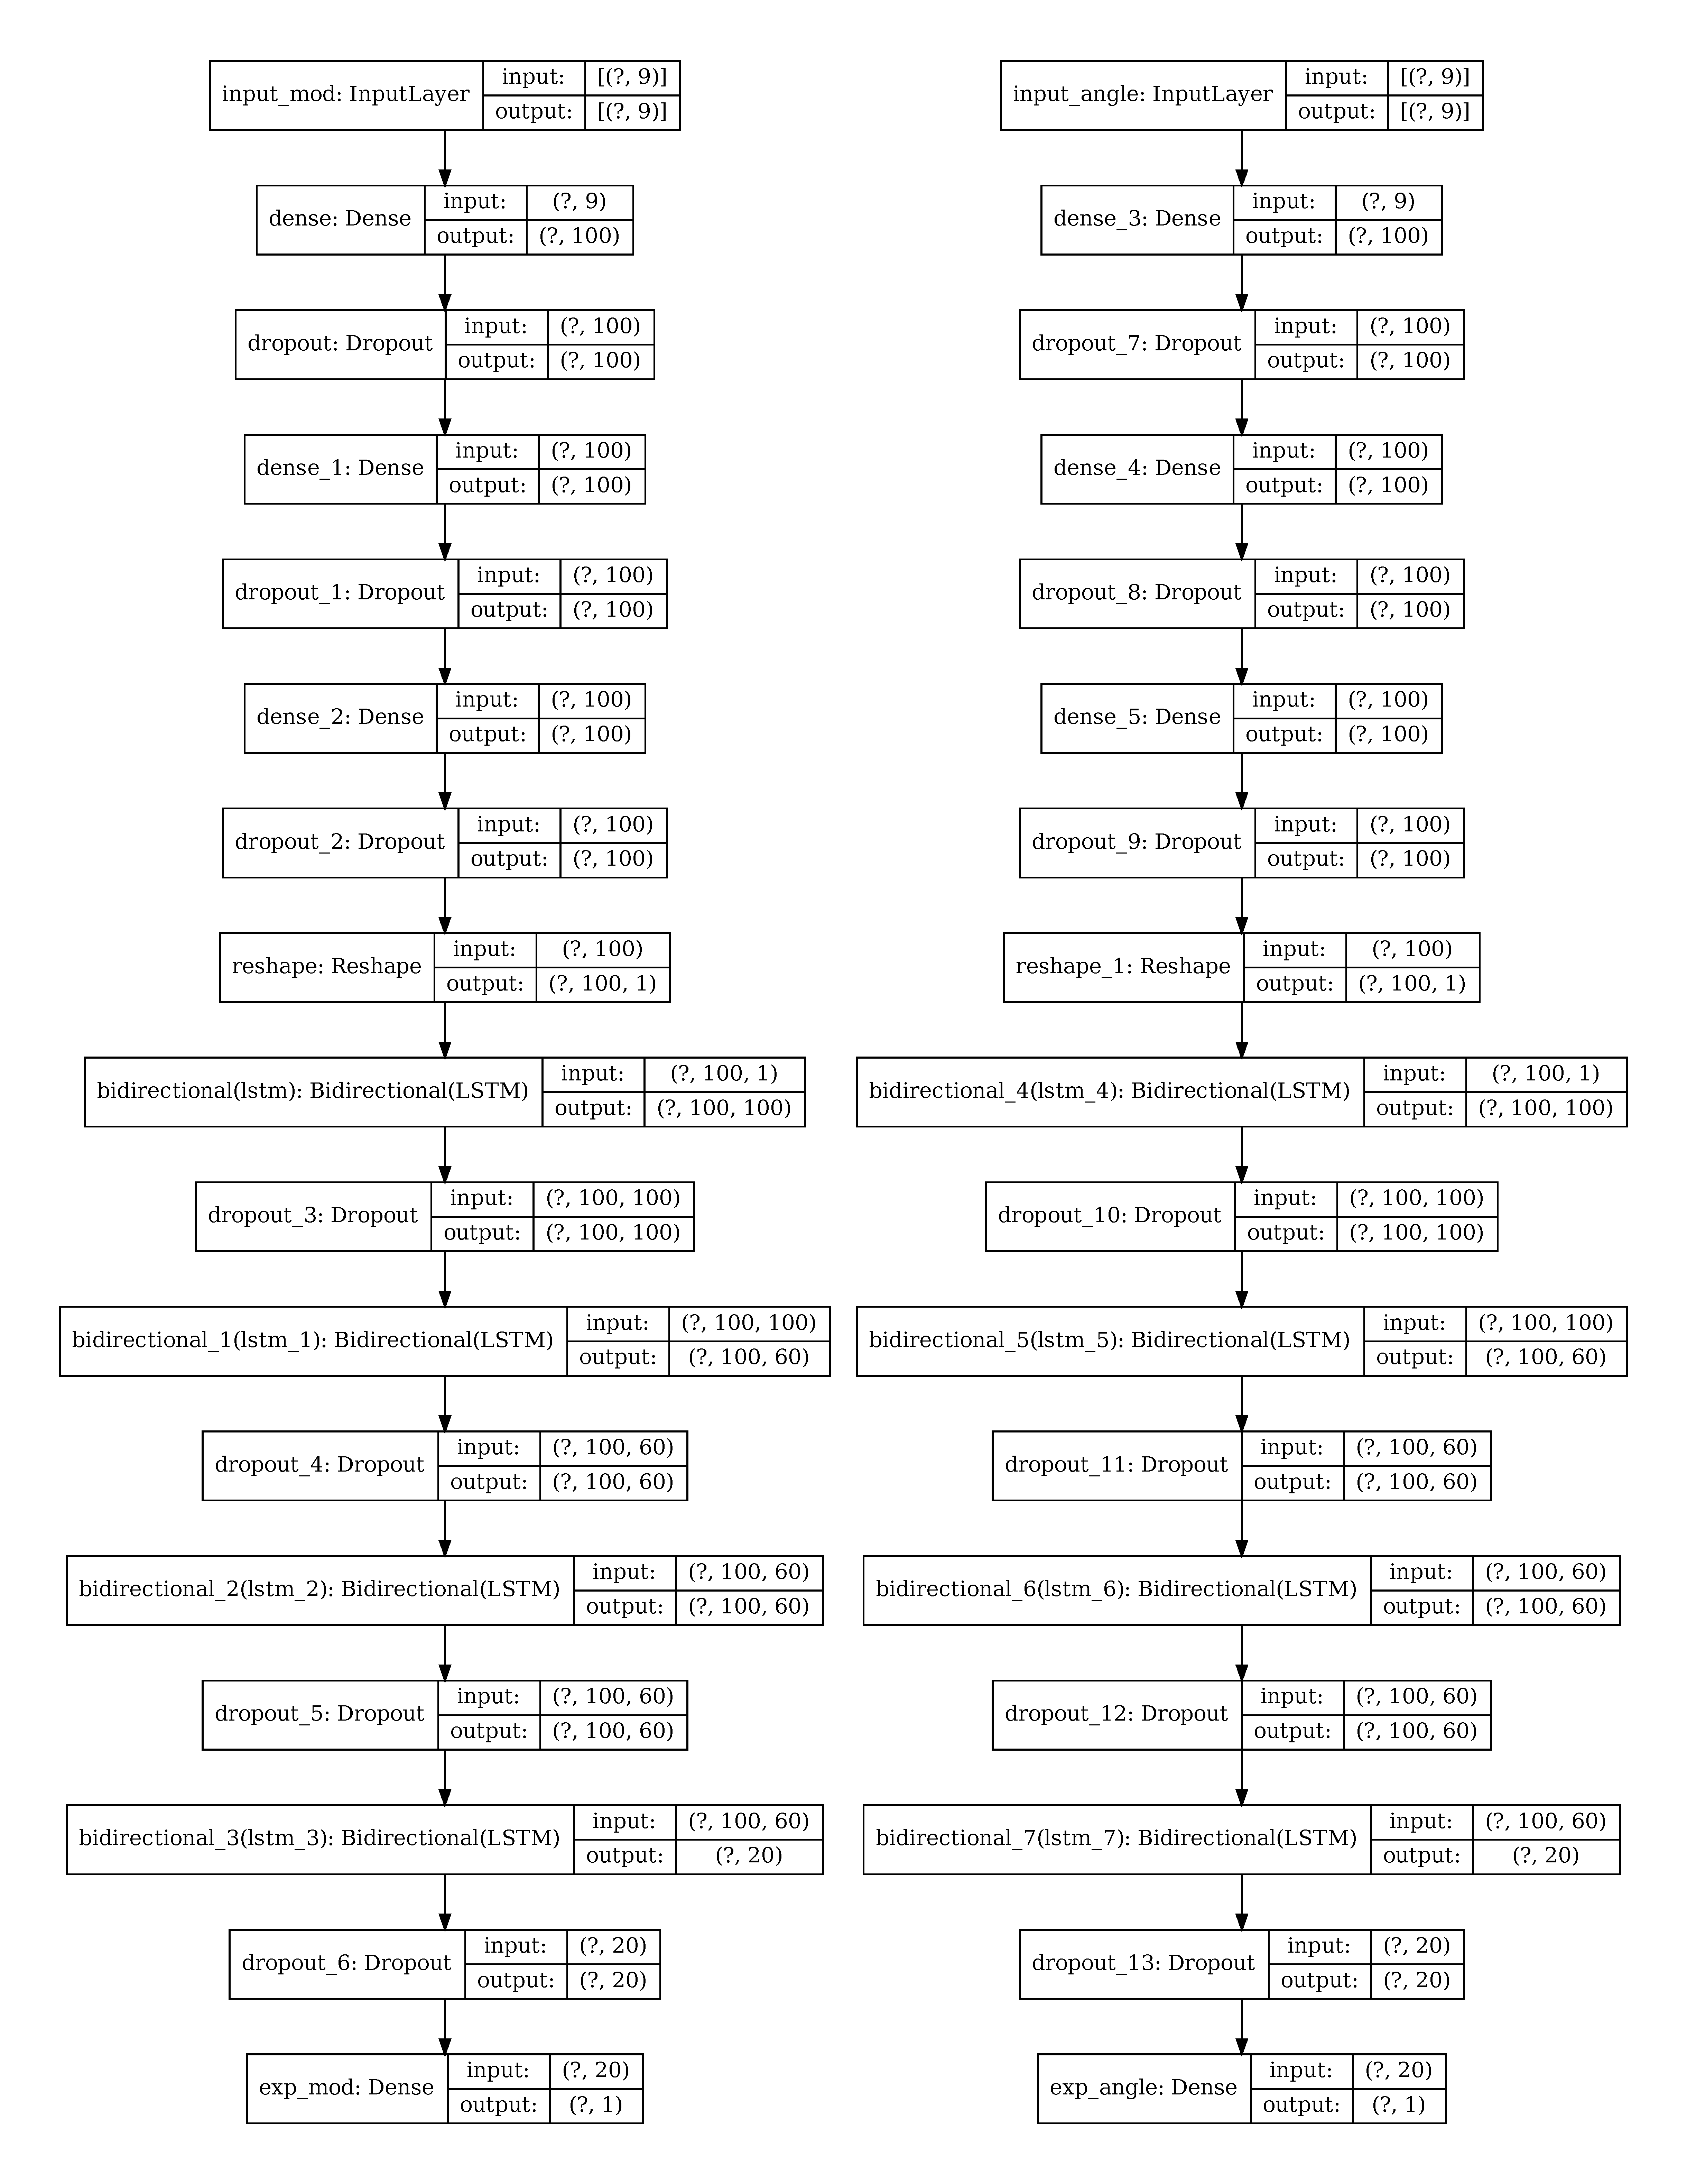
\includegraphics[width=0.45\linewidth]{img/wzw_ann_arch_lstm}
  \caption{Traditional LSTM.}
  \label{fig:wzw:lstm_trad}
\end{figure}

\begin{figure}[htbp]
  \centering
  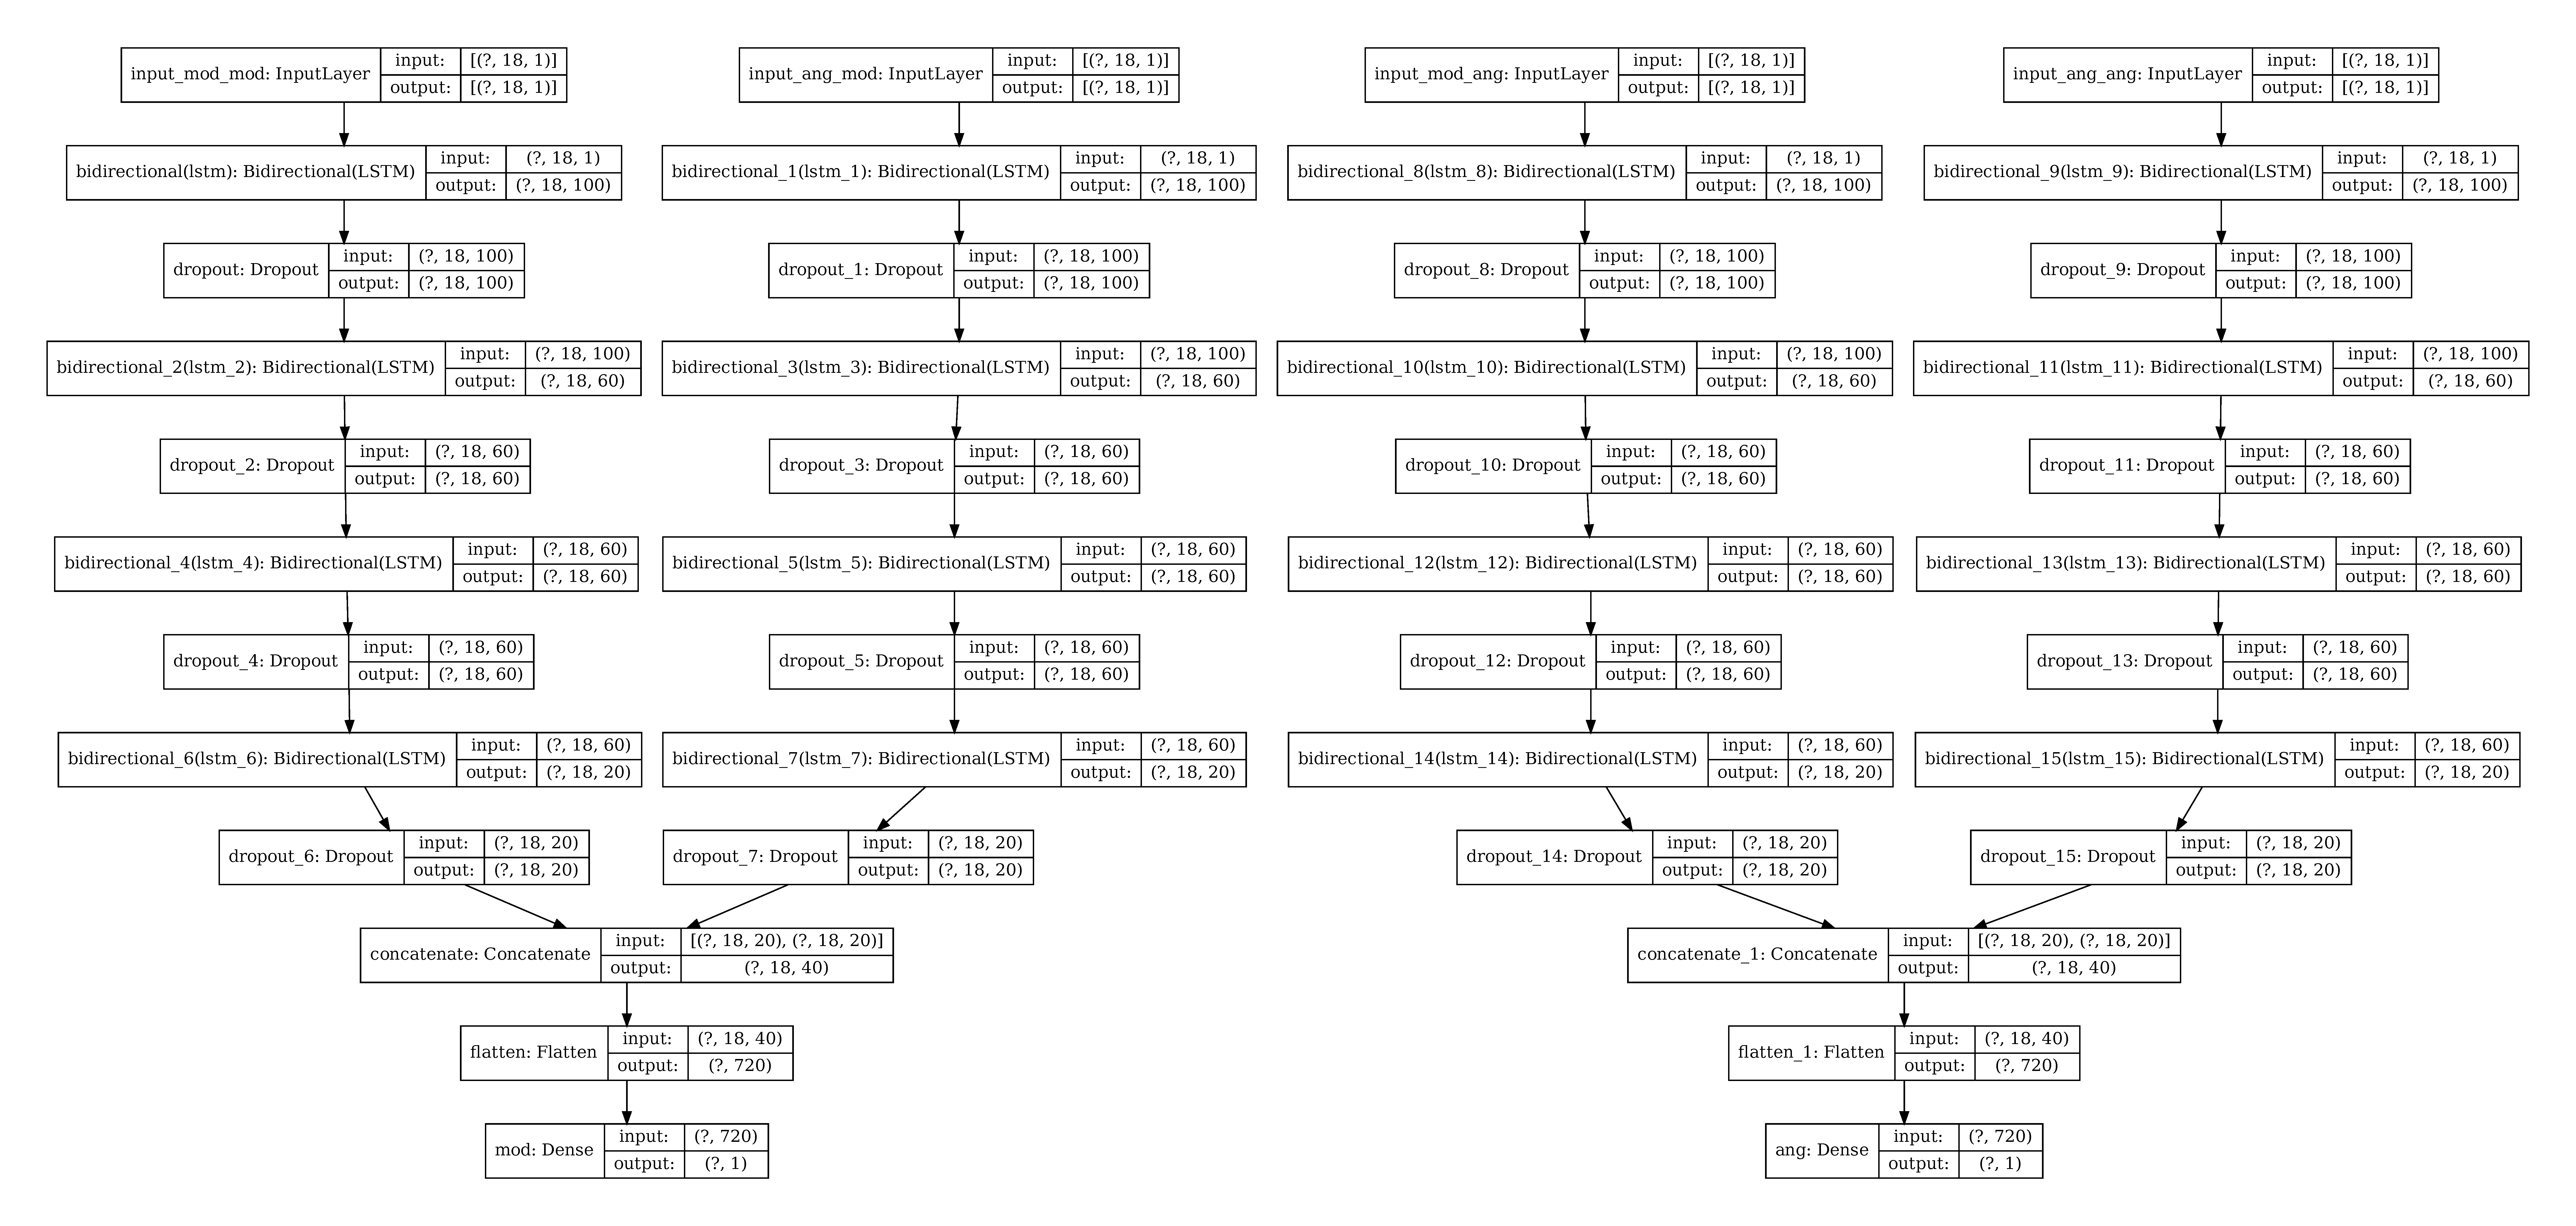
\includegraphics[width=0.95\linewidth]{img/wzw_ann_arch_lstm_fft}
  \caption{Fourier transformed LSTM.}
  \label{fig:wzw:lstm_fft}
\end{figure}

In this part of the analysis we train two separate LSTM models: the first separately takes the complex modulus of the truncation levels to predict the modulus of \texttt{exp} and their argument angles to predict \texttt{exp} (see~\Cref{fig:wzw:lstm_trad}), while the second takes the complex modulus and the angles of the Fourier transformed truncation levels to separately predict the complex modulus and the angle of \texttt{exp} (notice in~\Cref{fig:wzw:lstm_fft} that the input is separated into two different parallel architectures to avoid sharing the weights of the layers.

The first architecture in~\Cref{fig:wzw:lstm_trad} is made of two similar parallel architectures of \num{4} bidirectional hidden LSTM layers of \numlist{50;30;30;10} units each.
A dropout rate of \num{0.2} was added after the first layer, while a dropout of \num{0.1} was used after each of the other LSTM layers.
We also used a $\ell_2$ kernel regularisation of $10^{-3}$ after in the first two layer of the complex modulus architecture and $10^{-4}$ everywhere else.
The model was compiled using the \texttt{Adam} optimiser with initial learning rate $lr_0 = 10^{-3}$.
A learning rate scheduler was used to reduce the learning rate according to \eqref{eq:lumps:lrschedule}.
An early stopping callback was used to halt the training after \num{2500} epochs without improvement in the validation loss function (\mse).

The second architecture (\Cref{fig:wzw:lstm_fft}) follows the same construction as the first with a $\ell_2$ regularisation of $10^{-3}$ in every layer.
The structure is however duplicated to use complex numbers as input to predict both the complex modulus and the angle of the label \texttt{exp}.
For each of the inputs the layers dealing with the complex modulus and the angles have been concatenated before the output layers.

\begin{table}[htbp]
  \centering
  \begin{tabular}{@{}ccccc@{}}
    \toprule
    & \mse & \mae & \rr & R \\
    \midrule
    LSTM (mod)         & 0.011 & 0.06 & 0.87 & -0.32 \\
    LSTM (angle)       & 0.003 & 0.03 & 0.87 & 0.11  \\
    LSTM + FFT (mod)   & 0.02  & 0.08 & 0.75 & -0.05 \\
    LSTM + FFT (angle) & 0.005 & 0.04 & 0.82 & 0.45  \\
    \bottomrule
  \end{tabular}
  \caption{Metrics of the LSTM architectures computed on the test fold of the WZW dataset.}
  \label{tab:wzw:lstmmet}
\end{table}

In~\Cref{tab:wzw:lstmmet} we show the metrics computed on the test fold of the WZW dataset.
It seems that LSTM recurrent networks can help in slightly improving the predictions of the complex modulus of the extrapolated labels.
However the argument angles are not better than using the finite truncation levels, even though they represent a major improvement with respect to the previous analysis.


\subsubsection{Additional Analyses and Complementary Data}

As in the case of the lumps dataset, it is possible to find more analyses on the WZW data on \href{https://github.com/thesfinox/ml-sft-trunc/tree/model-dep}{GitHub}.
The repository stores notebooks containing analyses going in parallel to the lumps dataset, subsampling the WZW data according to \texttt{type} and \texttt{weight} as well as by their ``good'' behaviour (see~\Cref{sec:lumps:other} for a complete description).\footnotemark{}
\footnotetext{%
  For simplicity we call ``well behaving'' the samples whose absolute difference of the label \texttt{exp} with the last finite truncation level (\texttt{level\_10} in this case) is $\le 0.1$.
}
Interestingly we can see that in the case of the WZW dataset the well behaving samples show a good improvement using the LSTM network.
In fact the $R$ metric using those samples is \num{-0.45} for the complex modulus of \texttt{exp} and \num{-0.55} for its angle.
The bad results in~\Cref{tab:wzw:lstmmet} are therefore entirely due to the other samples, which in general correspond to higher values of the \texttt{weight} variable.

% vim ft=tex
